\documentclass{article}

\usepackage[a4paper]{geometry} % document dimensions
%\usepackage{amsmath} % multiline equation numbering
\usepackage{amssymb} % e.g. triangleq, checkmark
\usepackage{textcomp,gensymb} % \degree symbol
%\usepackage{bm} % bold symbols numbering
\usepackage{authblk} % author/affiliation block
\usepackage[T1]{fontenc} % support accents via UTF
\usepackage[titletoc,title]{appendix}
\usepackage{booktabs} % e.g. \toprule

\usepackage{graphicx} % support for graphics
\usepackage[hidelinks, backref=page]{hyperref} % hyperlinks and autoref
\hypersetup{
    pdfauthor={Nick Ackerley},
    pdfsubject={Engineering Seismology},
    pdftitle={An Open Model of Probabilistic Seismic Hazard Assessment for the Indian Subcontinent},
    pdfkeywords={seismology, hazard, India, OpenQuake}}
\usepackage{natbib} % bibliography support
\usepackage{adjustbox} % support for too-wide figures
\usepackage{caption} % support for captions of floats
\usepackage{capt-of} % support for captionof
\usepackage{subcaption} % support for multiple figures with captions
\providecommand*\hyphen{-} % dashed page numbers in bib
\usepackage{listingsutf8} % for syntax-highlighted code
\usepackage[usenames,dvipsnames]{xcolor} % e.g. RoyalBlue
\usepackage{fontspec} % support for setmonofont
\setmonofont{Ubuntu Mono}[Scale=MatchUppercase]

%\usepackage{multirow} % cells spanning rows in \crefs
%\usepackage{array} % vertically aligned table cells

\usepackage{enumitem} % control list formatting
\setlist[2]{nosep}

% allow figures to take up more of a page
\renewcommand{\floatpagefraction}{0.7}

% just call everything a "section", except an "appendix"
\renewcommand*{\sectionautorefname}{Section}
\renewcommand*{\subsectionautorefname}{Section}
\renewcommand*{\subsubsectionautorefname}{Section}
\newcommand*{\Appendixautorefname}{Appendix}

% set up back-references
\renewcommand*{\backref}[1]{}
\renewcommand*{\backrefalt}[4]{%
    \ifcase #1 (Not cited.)%
    \or        (Cited on page~#2.)%
    \else      (Cited on pages~#2.)%
    \fi}

\lstdefinelanguage{Ini}
{
    basicstyle=\ttfamily\footnotesize,
    breaklines=true,
    keepspaces=true,
    columns=fullflexible,
    morecomment=[s][\color{RoyalBlue}\bfseries]{[}{]},
    morecomment=[l]{\#},
    morecomment=[l]{;},
    commentstyle=\color{gray}\ttfamily,
    morekeywords={},
    otherkeywords={=,:},
    keywordstyle={\color{green}\bfseries},
}

%%% PREAMBLE

\begin{document}

\title{An Open Model of Probabilistic Seismic Hazard Assessment for the Indian Subcontinent}
\date{\today}

\setcounter{Maxaffil}{0} % compact author block
\author[1,2]{N. Ackerley}
%\author[3]{G. Weatherill}
%\author[3]{M. Pagani}
\affil[1]{Istituto Universitario di Studi Superiori, Pavia, Italy}
\affil[2]{Université Joseph Fourier, Grenoble, France}
%\affil[3]{Global Earthquake Model (GEM), Pavia, Italy}

\maketitle

\begin{abstract}
Open models encourage peer review and collaboration; open models can be built upon.
\end{abstract}

\tableofcontents
\listoffigures
\listoftables

\section{Introduction}
\label{sec:Introduction}

In this work a seismic hazard model for peninsual India \cite{nath2012probabilistic} is implemented within the OpenQuake \citep{weatherill2014openquake,crowley2015openquake} platform.

This report is intended to be archived with the input and output files necessary to replicate the results at \url{https://hazardwiki.openquake.org/}. References to file names in the electronic data are shown in \texttt{typewriter} font, as are keywords specific to OpenQuake, such as \texttt{bGRRelative}.

\subsection{Seismic hazard in the Indian subcontinent}
\label{subsec:PshaIndia}

Seismic hazard in India has of course been studied extensively, progressing from deterministic studies to probabilistic seismic hazard assessment (PSHA) and from site-specific to regional studies. \cite{ashish2016probabilistic} gives an up-to-date overview of the importance and history of this work. Of particular note is the fact that the Bureau of Indian Standards has not updated their seismic hazard zonation since 2002 \citep{bis2002criteria}. \cite{nath2012probabilistic} summarizes concerns with the standard currently in force.

Some studies have focused on the extreme hazard of the Himalayas \citep{Bilham2001} in the the northeast, including the Shillong plateau, \citep{Das2006} and northwest \citep{Mahajan2009}. Other studies have focused on regions of lesser but nonetheless high hazard such as Gujarat \citep{Yadav2008} or considered the whole of stable ``peninsular India" \citep{jaiswal2007, ashish2016probabilistic}. Only \cite{bhatia1999probabilistic} considered the whole of India, but as \cite{ashish2016probabilistic} points out, since it was part of a global hazard mapping project (GSHAP) it only included ``only a few sources for Peninsular India focusing on the inter-plate
region along the Himalayan belt".   

\cite{nath2012probabilistic} is thus distinguished from previous work in providing a detailed probabilistic hazard assessment for the whole of India, including neighbouring states such as Bangladesh and Nepal. It is the culmination of several previous works, some unpublished, involving the same group of authors. These works include development of a uniform catalogue \citep{nath2010earthquake}, development of GMPEs specific to the Shillong region \citep{nath2012ground}, evaluation of a suite of GMPEs applicable to India \citep{nath2011peak} and development of smoothed-gridded and areal seismicity models \citep{thingbaijam2011seismogenic}. Although there are inevitably some limitations, as we shall see later, this work represents the current state-of-the-art as far as PSHA in India.

(In the discussion of possible improvements to \cite{nath2012probabilistic} it will be noted that while earlier investigations \citep{bhatia1999probabilistic, Das2006, Yadav2008, jaiswal2007} relied on areal seismogenic source zonation, \cite{nath2012probabilistic} adds smoothed-gridded point sources while \cite{ashish2016probabilistic} adds fault-modelling. Different types of seismogenic zones address different types of hazard and return periods, and can be effectively combined using logic trees to better encapsulate epistemic uncertainty.)

\subsection{Open science and OpenQuake}
\label{subsec:Open}

The seismological research community is a collegial one and, as they must, researchers generally share data, models, software and results freely. However it is becoming a generally recognized problem that scientific computation, even as significant technological advances are made, is falling far short of expectations in terms of reproducibility.

Reproducibility is one of the fundamental tenets of science. In other disciplines, the components of a properly-documented experiment are well-known and widely practiced. Scientific computing is a relative newcomer, and presents new challenges, such as the constant evolution of programming languages.

Although \cite{nath2012probabilistic} provides much of the information necessary to reproduce their results as an electronic supplement, it is incomplete, and worse, the software used to run the simulations is not freely available. The consequence is that results cannot be verified, errors cannot be corrected and improvements cannot be made.

The OpenQuake \citep{crowley2015openquake} is a fully-featured suite of software for the modelling of seismic hazard and risk. The source code is open, freely distributable and modifiable. It is an ideal platform for development of PSHA model. In fact, there is an ongoing effort to build a Global Earthquake Model based on OpenQuake.

Essential components of reproducibility: model data (completely documented), result data (completely documented), freely available software (version numbers, repository commits), hardware capable of running the software.



\subsection{Overview}
\label{subsec:Overview}

In \autoref{sec:Implementation} the process followed to translate the model of \cite{nath2012probabilistic} for OpenQuake is detailed. Specific issues around tectonic region assignments are addressed in \autoref{subsubsec:Areal}. Difficulties encountered in interpreting and implementing the smoothed-gridded seismicity models are detailed in \autoref{subsubsec:Smoothed} while recommendations for an improved smoothed-gridded model are made in \autoref{appendix:Catalogue}.

In \autoref{subsec:GroundMotion} issues encountered in implementing ground motion prediction equations are discussed.

\autoref{subsec:LogicTrees} discusses the development of the logic trees. Some inconsistencies were encountered in the application of previous research regarding the usage of GMPEs in India. This is discussed briefly in \autoref{subsubsec:GmpeTree} and recommendations for future work are made in \autoref{appendix:AlternativeGmpes}. The modelling of source frequency magnitude distribution uncertainty described in \cite{nath2012probabilistic} turned out to be unimplementable in the strictest sense in OpenQuake and possibly on any platform, so compromises made are described in \autoref{subsubsec:SourceTree}.

\autoref{subsec:Verification} verifies the current results against those of  \cite{nath2012probabilistic}. In particular hazard curves and maps and tables of ground motion with various probabilities of exceedence are presented and evaluated. Inconsistencies between the figures and electronic supplement of \cite{nath2012probabilistic} are discussed. \autoref{subsec:Sensitivity} investigates the importance of the use of region-specific ground motion prediction via their impact on hazard levels.

\autoref{subsec:Discussion} briefly explores the possibilities for future work while reserving more detailed discussion reserved for the appendices.

\section{Implementation}
\label{sec:Implementation}

\subsection{Seismogenic sources}
\label{subsec:Sources}

The electronic supplement of \cite{nath2012probabilistic} provides most but not all of the information required to generate a complete source model, even supplemented with the helpful additional information found in \cite{thingbaijam2011seismogenic}. This section thus focuses on bridging the gaps to construct a complete source model.

As shown in \autoref{fig:SourceTreeSymbolic}, \cite{nath2012probabilistic} actually proposed three source models, a single set of areal seismogenic source zones, and two smoothed-gridded point source models. Doing so retains benefits from both types of models without neglecting the related epistemic uncertainty model. Both models are derived from the catalogue of \cite{nath2010earthquake} for sub-catalogues with different minimum magnitudes and depth ranges.

\cite{thingbaijam2011seismogenic} divide their model into four layers as summarized in \autoref{table:Completeness} and \autoref{fig:DepthHistogram}. Crustal thicknesses vary significantly across the region of study, but the convenience of constant model layer thicknesses turns out to be not entirely unrealistic. The continental crust is 75-80 km thick beneath the Himalayas where the tectonics can be divided into shallow crust and interface \citep{thingbaijam2011seismogenic}. Similarly in the the Shillong plateau of Northeast India the crust is quite thick and significant variation of stress drop with depth has been noted, with devastating ``pop-up'' type events \cite{bilham2001plateau} being generated in the lower crust \citep{nath2012ground}. In stable continental regions the crustal thickness is a more usual 35-45 km, with seismicity concentrated in the uppermost 25 km. The preceding seismotectonic features can be represented reasonably well using two seismogenic layers: 0-25 km and 25-70 km. 

\begin{table}[tb]
\centering
\caption[Summary of layer characteristics used for source models.]{Summary of layer characteristics used for source models. Completeness magnitudes and years used in generating original smoothed-gridded seismicity models are from Table 1 of \cite{thingbaijam2011seismogenic}. Layer identifiers used throughout this report are indicated. Tops and bottoms of layers have been taken as seismogenic depth limits. Hypocentral depths listed are at mid-layer.}
\label{table:Completeness}
\begin{tabular}{cccccccccc}
\multicolumn{4}{c}{minimum magnitude} & \multicolumn{2}{c}{4} & \multicolumn{2}{c}{4.5} & \multicolumn{2}{c}{5.5} \\
\midrule
layer & \multicolumn{3}{c}{
\begin{tabular}{ccc}
\multicolumn{3}{c}{depth (km)}\\min. & max. & hypo.\\
\end{tabular}
} & start & end & start & end & start & end \\
\midrule
1 & 0   & 25  & 12.5 & 1994 & 2008 & 1964 & 2008 & 1903 & 2008 \\
2 & 25  & 70  & 47.5 & 1990 & 2008 & 1964 & 2008 & 1902 & 2008 \\
3 & 70  & 180 & 125  & 1996 & 2008 & 1964 & 2008 & 1914 & 2008 \\
4 & 180 & 300 & 240  & 1970 & 2008 & 1984 & 2008 & 1912 & 2008 \\
\bottomrule
\end{tabular}
\end{table}

Intra-slab subduction occurs in three broad zones: the Hindu-Kush and Pamir ranges in the north-west, the Indo-Myanmar subduction zone in the north-east and the Sumatra-Andaman subduction zone in the south east. Deep-seated seismicity only occurs in the first and last region. The tectonics of the Indo-Myanmar region are a combination of oblique subduction, accretion and collision \cite{wang2014active}. These tectonic zones are represented by two deeper seismogenic layers: 70-150 km and 150-300 km.

This stack of depth-limited seismogenic zones can crudely represent the fact that subduction events are generally spread over a dipping plane (see \autoref{fig:DepthVsDistance}). The four-layer structure furthermore captures the fact that there are 4 clear modes in the distribution of depths (see \autoref{fig:DepthHistogram}). 

\subsubsection{Areal zones}
\label{subsubsec:Areal}

Areal source models are appropriate when source mechanisms and seismicity rates are relatively constant across the area, and can provide a sound basis for regional variation of b-value, maximum magnitude and other key parameters of a frequency-magnitude distribution. 

As we will see in \autoref{subsubsec:GmpeTree} ground motion prediction logic trees depend on correct assignment of tectonic region types. The main difficulty in implementing the areal source model of  \cite{nath2012probabilistic} was that although their intentions were generally clear, these region assignments were not made explicit. Tectonic region type assignments were therefore made using a combination of the representative focal mechanisms reported by \cite{nath2012probabilistic} and fault maps such as the HimaTibetMap database \citep{styron2010database}. Since the representative focal mechanism was computed as the average of the moment tensors reported in the GCMT database weighted by magnitude it is biased in favour of the larger earthquakes \citep{thingbaijam2011seismogenic}. The inferred tectonic region assignments assumed are shown in \autoref{fig:ArealSourceModel}.

\begin{figure}[!htb]
\begin{adjustbox}{center}
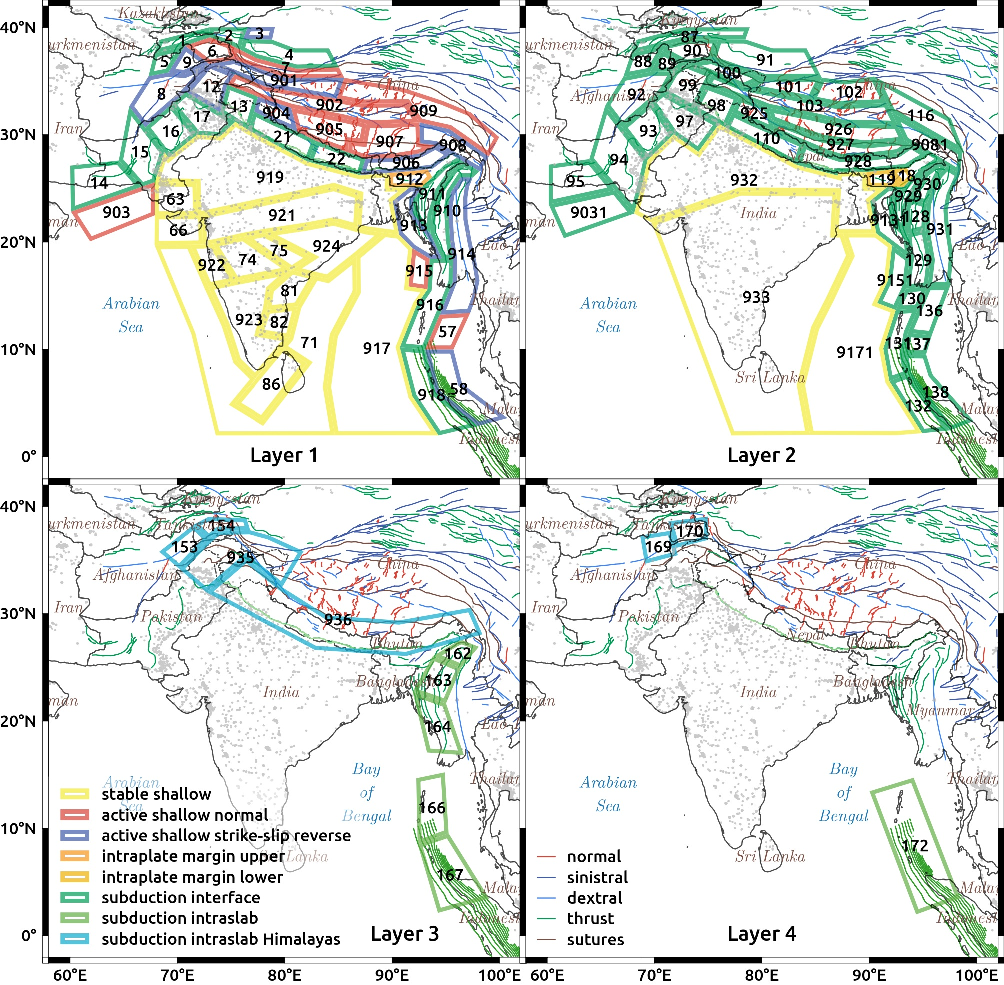
\includegraphics{India_Areal_Source_Model}
\end{adjustbox}
\caption[Areal source model]{Areal source model tectonic region assignments used in GMPE logic tree. The areal source models is encoded in \texttt{\detokenize{areal_source_model.xml}}. Zone identification numbers from \cite{nath2012probabilistic} are indicated. Fault traces are from HimaTibetMap-1.0 \citep{styron2010database} except the Sumatran subduction fault which is from SLAB~1.0 \citep{hayes2012slab1}. Fault data from the stable regions of India is lacking. Urban areas, ``contiguous patches of built-up land greater than 1~km²'' \citep{schneider2009new}, are indicated in darker grey.}
\label{fig:ArealSourceModel}
\end{figure}

Potentially problematic tectonic region type assignments include:
\begin{itemize}
\item zone 906 in the Great Himalayas just north of the Shillong plateau was assigned ``active shallow crust strike-slip reverse'' even though the main trace of the Himalayan subduction fault runs through it, because the representative focal mechanism is strike-slip. 
\item zones 71, 86 on layer 1 and zones 9031, 9081, 9131, 9151 and 9171 on layer 2 have have $a$ values of zero and so were not included in the areal source model
\end{itemize}

Magnitude-scaling relations are used in PSHA to determine the actual rupture dimensions once a magnitude has been drawn from a frequency-magnitude distribution. These were relatively straightforward to select once the tectonic region assignments were made, since ``Wells and Coppersmith (1994) for crustal events and those given by
Strasser et al. (2010) for the subduction earthquakes'' \citep[p.~140]{nath2012probabilistic}. For interface and intraslab regions \texttt{StrasserInterface} and \texttt{StrasserIntraslab} were used, respectively. The comment that ``the fault-rupture area estimated from the magnitude is constrained by a factor of 2'' \citep[p.~140]{nath2012probabilistic} was similarly interpreted as a width/depth aspect ratio of 2.

Since it is not explicitly stated in \cite{nath2012probabilistic} the seismogenic depth was assumed to be midway between the minimum and maximum for each layer. Potential refinements to this setup are discussed in \autoref{appendix:SourceModelImprovements}.

The supplementary information required to generate the fully specified areal source model from the electronic supplement files \texttt{polygonlay\%d.txt} and \texttt{seismicitylay\%d.txt} files in the is contained in \texttt{auxiliary data.csv}.

\subsubsection{Smoothed-gridded}
\label{subsubsec:Smoothed}

Smoothed-gridded seismicity models aim to replicate geographic variations of activity rates in a catalogue-driven way. Typically a smoothing kernel is used which enforces a correlation distance and limits the resolution.

After some discussion with the second author it was decided that although the models are described as ``spatially varying annual activity rates'' \cite[p.~140]{nath2012probabilistic} the electronic supplement actually contains spatially smoothed total seismicity, i.e. number of events (per cell). In order to convert this information to activity rates, i.e. number of events per year (per cell), it was necessary to obtain the duration of each sub-catalogue. Fortunately the missing ingredient is summarized in \cite[Table 1]{thingbaijam2011seismogenic} and reproduced in \autoref{table:Completeness} below.

In OpenQuake each point in the smoothed seismicity model is treated as a point source with a specified frequency-magnitude distribution: at a minimum $a$, $b$ and $M_{max}$ must be spedified. \cite{nath2012probabilistic} indicate that ``b-value and m max remain fixed within the source zone''. Thus for the smoothed seismicity model the parameters $b$ and $M_{max}$ of the truncated Gutenberg-Richter magnitude-frequency distributions are to be inferred from the areal source model zonation. For points inside zones with non-zero $a$ values in the areal source model this is trivial; for points outside these zones the zone with the shortest perpendicular distance was chosen.

A point source model in OpenQuake also requires definition of the uncertainty of the probability distribution, as well as the tectonic region type and source mechanism for the selection and implementation of GMPEs, respectively. Thus the same procedure was used to assign $\sigma_b$, $\sigma_{m_{max}}$, tectonic subregion, rake, dip, strike and magnitude scaling relations were used.

The electronic supplement to \cite{nath2012probabilistic} for the smoothed-gridded seismicity models simply gives values for \texttt{\detokenize{nu4_5}} and \texttt{\detokenize{nu5_5}} for each latitude and longitude, where ``$\nu_i$ , is the annual activity rate for $i$th seismogenic source for a threshold magnitude'' \cite[p.~140]{nath2012probabilistic}.

The truncated Gutenberg-Richter magnitude-frequency distribution in OpenQuake implements
$$\lambda(M \geq m) = 10^{a - b m} = e^{\alpha - \beta m}$$
where, since $\lambda$ is an annual rate, $10^a$ is too. If we ignore events below some threshold $m_{min}$ then the annual rate becomes
$$\lambda(M \geq m_{min}) = e^{\alpha - \beta m_{min}} e^{-\beta (m - m_{min})} = \nu e^{-\beta (m - m_{min})} $$
Thus to compute the $a$ value required by OpenQuake from the activity rate $\nu$ for a given magnitude threshold, we must also take into account the $b$ value for the zone:
$$a = \log_{10}(\nu) + b m_{min}$$
Applying this formula gives rates for the areal model which agree well with the catalogue, but the rates in the smoothed-gridded seismicity model are on the order of 100x higher. Figure 3.6 of \cite{thingbaijam2011synoptic} shows rates in line with those of \cite{thingbaijam2011seismogenic} and which better agree with the areal rates. In discussion with the author was concluded that the electronic supplement to \cite{nath2012probabilistic} is in error.

\begin{table}
\caption[Comparison of seismicity rates]{Comparison of seismicity rates in areal and smoothed-gridded seismicity models to those obtained from the catalogue.}
\label{table:Rates}
\centering
/home/nick/Desktop/Individual Study/Source Models/activity_rates_by_layer_areal_vs_smoothed_vs_catalogue.tex
\end{table}

\begin{figure}[!htb]
\begin{adjustbox}{center}
\includegraphics{India_Smoothed_Source_Model}
\end{adjustbox}
\caption[Smoothed seismicity point source model]{Tectonic region assignments and activity rates for smoothed seismicity point source model. The smoothed seismicity source models are encoded in \texttt{\detokenize{smoothed_source_model_mmin4.5.xml}} and \texttt{\detokenize{smoothed_source_model_mmin5.5.xml}}}
\label{fig:SmoothedSourceModel}
\end{figure}

Other assumptions:
\begin{itemize}
\item zones 9031, 9081, 9131, 9151 and 9171 on layer 2 have $m_{max}$ values values of zero so the the smoothed seismicity points in or nearest to these zones on layer 2 were assigned the $m_{max}$ values from the corresponding zones on layer 1, namely zones 903, 908, 913, 915 and 917.
\end{itemize}

Note differences in grids: although the hazard maps in the electronic supplement are at 0.2° and the paper says the smoothed-gridded models are also at 0.2° they are in fact at 0.1°. Figure shows the model at just 0.2°.

Note smoothing details. A Gaussian kernel is used, following the methodology of \cite{frankel1995mapping} with correlation distances of 65 and 85~km for $m_{min}$ of 4.5 and 5.5 respectively. The method involves smoothing event counts, thus events per year, for a given minimum magnitude.

\cite{thingbaijam2011synoptic}

\cite{nath2010earthquake}

\subsection{Ground-motion prediction}
\label{subsec:GroundMotion}

Importance of models implemented for this study. 

The great Assam earthquake of 1897 destroyed buildings within several hundred km. The two main fault structures involved are capable of M > 8 plateau-building events with a recurrence interval of 3-8 kyr each \citep{bilham2001plateau}.

\cite{nath2012ground} notes stress drop apparently increasing with depth and models $\kappa$ using a database of recent well-recorded micro-earthquakes, and uses this information to develop stochastic models for events in the upper and lower crust. The simulations are of vertical motion at a hard-rock site and no site corrections are attempted.

\cite{sharma2009ground} points out that the decay rate of PGA for shallow India-Bangladesh and deep India-Burma border events have different distance scaling. The former leads to the necessity of a GMPE specific to the Shillong plateau \cite{nath2012ground} while the latter means interface subduction events need to be treated differently. 

Issues encountered while implementing GMPE logic tree:
\begin{itemize}
\item layer~4 depth range of 180-300~km is significantly deeper than deepest events used in regression for ATBO03 (100 km), LILE08 (161 km), ZHAO06 (120 km) and GUPT10 (148 km) are specified for. YCSH97 only included events to 229 km. KANN06 is specified to 200 km depth, but is only used for interface events (layer~2).
\item Assumed “and Andaman-Sumatra subduction” missing from Figure 3.
\item Why is Youngs (1997) not used in the subduction interfaces?
\item Should the Japan/Cascadia distinction not also be used for interface subduction with Atkinson \& Boore (2003)?
\item \cite{nath2012probabilistic} doesn't seem to me to follow the recommendations of \cite{nath2011peak} as far as having two subduction intra-slab sub-regions: the former uses Indo-Myanmar and Himalayas while the latter recommends Indo-Myanmar and Hindukush. \cite{nath2012probabilistic} is followed strictly for for phase 1.
\item Assignment of source mechanism (normal or not, matters in shallowest layer only) is tricky.  Dip cannot be used to distinguish normal and reverse subduction because the subduction interface angle is not known. different GMPEs use different rake thresholds; a threshold of 30\degree\space was chosen, consistent with \cite{boore2008ground, campbell2008nga} but not \cite{zhao2006attenuation}.
\end{itemize}

Issued encountered while implementing GMPEs:

\cite{sharma2009ground}
\begin{itemize}
\item lacks a $M^2$ term \cite{cotton2006criteria}
\item does not define rock vs. soil
\end{itemize}

\cite{raghukanth2007estimation}
\begin{itemize}
\item typographical errors in coefficient tables: grossest error fixed, 3 other errors causing approximately 10\% error not fixed
\item actually defines 4 different models: must assume that for all of peninsular India was used by \cite{nath2012probabilistic}, not one of those for sub-regions.
\end{itemize}


\begin{table}
\caption[Ground motion prediction equations]{Ground motion prediction equations. Models newly implemented in OpenQuake as part of the current work are indicated.}
\label{table:GMPE}
\centering
\begin{tabular}{c c l}
\hline
 Code & New & Reference \\
\hline
 AKBO10 & & \cite{akkar2010empirical} \\
 BOAT08 & & \cite{boore2008ground} \\ 
 CABO08 & & \cite{campbell2008nga} \\ 
 ZHAO06 & & \cite{zhao2006attenuation} \\ 
 ATBO03 & & \cite{atkinson2003empirical} \\ 
 ATMA09 & & \cite{atkinson2009predicted} \\ 
 LILE08 & & \cite{lin2008ground} \\ 
 YCSH97 & & \cite{youngs1997strong} \\ 
 TORO02 & & \cite{toro2002modification} \\ 
 ATBO06 & & \cite{atkinson2006earthquake} \\ 
 CAMP03 & & \cite{campbell2003prediction} \\ 
 SDBK09 & \checkmark & \cite{sharma2009ground} \\
 RAIY07 & \checkmark & \cite{raghukanth2007estimation} \\
 NTMN12 & \checkmark & \cite{nath2012ground} \\
 GUPT10 & \checkmark & \cite{gupta2010response} \\
 KNMF06 & \checkmark & \cite{kanno2006new} \\
\hline
\end{tabular}
\end{table}


\cite{kanno2006new} -> \cite{douglas2003earthquake}

\subsection{Logic Trees}
\label{subsec:LogicTrees}

\subsubsection{Ground-Motion Prediction}
\label{subsubsec:GmpeTree}

The GMPE logic tree implemented in \cite{nath2012probabilistic} is shown in \autoref{fig:GmpeTreeNath}. Since some of these GMPEs are new to OpenQuake (see \autoref{table:GMPE}) a comparison was done between that model and that obtained with only the standard GMPEs. For this purpose a "simplified" GMPE logic tree was constructed which simply omitted the newly-implemented GMPEs and retained equal weighting for the rest.

\begin{figure}[!htb]
\begin{adjustbox}{center}
\includegraphics{gmpe_logic_tree_omit_new.pdf}
\end{adjustbox}
\caption[Simplified GMPE logic tree]{Simplified GMPE logic tree employing only established OpenQuake models, as encoded in \texttt{\detokenize{gmpe_logic_tree_omit_new.xml}}. Middle column selects tectonic region types as defined in \autoref{fig:ArealSourceModel}. OpenQuake model class names and assigned weights are given on the right side. New and established models are enumerated in \autoref{table:GMPE}}
\label{fig:GmpeTreeSimplified}
\end{figure}

\begin{figure}
\begin{adjustbox}{center}
\includegraphics{gmpe_logic_tree.pdf}
\end{adjustbox}
\caption[Original GMPE logic tree]{GMPE logic tree of \cite{nath2012probabilistic}, as encoded in \texttt{\detokenize{gmpe_logic_tree.xml}}. See \autoref{fig:GmpeTreeSimplified} for complete description}
\label{fig:GmpeTreeNath}
\end{figure}

Moving forward an obvious modification is to replace superseded NGA models with their more up-to-date versions. 

[It may also be desirable to rationalize the weighting of the GMPEs or include entirely new ones, such as the new BC Hydro subduction model \citep{abrahamson2012bc}. The discussion continues below and is incomplete.]

\cite{anbazhagan2015selection} seem to be proposing different weights for different regions based on single events in those regions. An extreme example is to define different weights for Anjar, 1956 and Bhuj , 2001 earthquakes even though the epicentres and depths were very close together. In contrast \cite{nath2011peak} compute LLH for 7 regions (using 38 events total) and state that, ``individual events do not have significant number of observations to support a viable ranking basis.''

\cite{anbazhagan2015selection} seem to misuse the concept of data support index (DSI) \citep{delavaud2012toward} by setting weights to zero when the DSI is negative. The threshold is arbitrary and is chosen without discussion. As \cite{delavaud2012toward} point out ``more important
than the sign of the DSI is the difference of DSI between
two models.''

Both \cite{anbazhagan2015selection} and \cite{nath2011peak} rely on estimating ground motions from macroseismic intensity. I'm sure it is a matter of low seismicity and lack of instrumentation, but I'm still surprised. I would expect the catalogue for peninsular India to be complete for 20 years to magnitude 5 so that one could thus get 10 well-recorded events, at least. There is significant additional (aleatory and epistemic) variability in mapping EMS to PGA which must obscure the true performance of the GMPEs.  Perhaps this is part of why  \cite{anbazhagan2015selection} and \cite{nath2011peak} arrive at such different LLH scores and rankings for the same events \cite[][Table 5]{anbazhagan2015selection}. It would be interesting to compare the results of LLHs computed using EMS inferred from digitized intensity maps to those computed using instrumental PGA for at least a few events since 1990. \cite{nath2011peak} take a step towards this by looking at the scatter in their mapping of PGA to EMS but it's not quite the same.

Many authors \citep{scherbaum2009model, nath2011peak, delavaud2012toward, anbazhagan2015selection} seem unduly interested in "ranking", i.e.  constructing an ordered list of GMPEs. This is not a horse race. \cite{scherbaum2009model} suggests a way to turn an LLH score into a logic-tree weight and the formula does not require ranking. Furthermore, in constructing a logic tree one must include factors outside the performance-based scoring, for example an assessment of whether the set is ``mutually exclusive and collectively exhaustive'' \citep{bommer2008use}. For me the question of ranking is just "noise" which obscures more important questions.

The mutual exclusivity requirement means, to me, that models should be omitted which are redundant in the sense of being too similar to other models in terms of the methodology of their construction, especially if that means they make similar predictions and have similar limitations as a result. For example the exclusion of models which have been superseded \citep{cotton2006criteria} can be seen as an application of the requirement that models be mutually exclusive. Another example would be, for a GMPE logic tree intended for the Indian subcontinent, to omit a model such as \cite{hwang1997attenuation} in favour of \cite{atkinson2006earthquake} since both are based on stochastic simulation in Eastern North America.

The collective exhaustiveness requirement means, is trickier. It is this requirement which pushes hazard modellers to seek out and evaluate more and complementary types of models. Thus models with broad data support from other regions complement models with poor data support from the target region. Stochastic models supplement data-driven models. Models with different functional forms, distance or magnitude ranges can complement each other.

The process of developing a logic tree to assess epistemic uncertainty is thus a dialectical one. Mutual exclusivity and collective exhaustiveness comprise opposing forces which must be exerted alternately and in tandem.

[Now apply these principles to move forward from \cite{nath2012probabilistic}!] 

\subsubsection{Source Models}
\label{subsubsec:SourceTree}

The source model logic tree is shown in symbolic form in \autoref{fig:SourceTreeSymbolic}.

\begin{figure}[!htb]
\begin{adjustbox}{center}
\includegraphics{source_model_logic_tree_symbolic.pdf}
\end{adjustbox}
\caption[Symbolic source model logic tree]{Symbolic source model logic tree of \cite{nath2012probabilistic}.}
\label{fig:SourceTreeSymbolic}
\end{figure}

\cite{nath2012probabilistic} accounts for the epistemic uncertainty in seismicity model parameters by estimating the standard deviations of $b$ and $m_{max}$ in each source zone and assigning weights to ±1 standard deviation for each source. This results in a source model logic tree too large to represent on a page; just a portion of it is shown in \autoref{fig:SourceTreePartial}. 

\begin{figure}
\begin{adjustbox}{center}
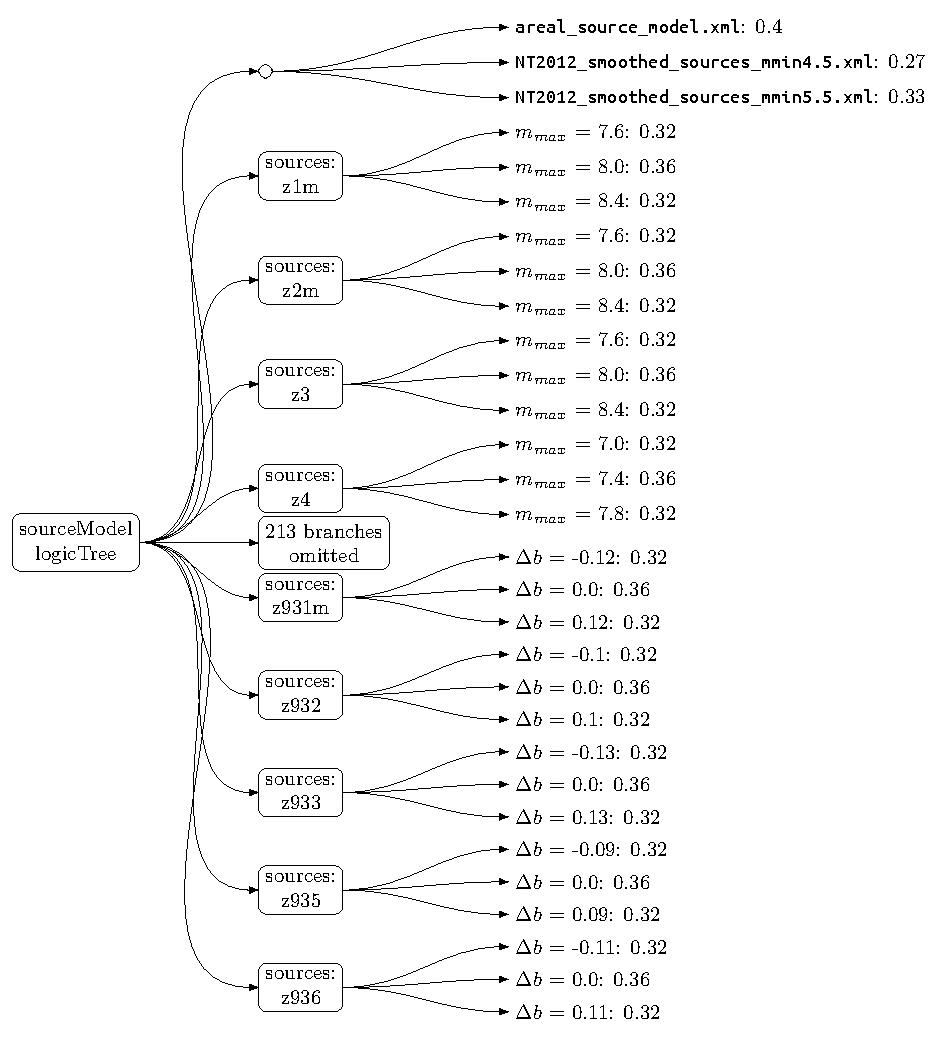
\includegraphics{source_model_logic_tree.pdf}
\end{adjustbox}
\caption[Partial source model logic tree]{Partial source model logic tree of \cite{nath2012probabilistic}. The full model is encoded in \texttt{\detokenize{source_model_logic_tree.xml}}}
\label{fig:SourceTreePartial}
\end{figure}

Note that although Figure 4 of \cite{nath2012probabilistic} shows the activity rate $\nu$ (and by implication $a$) varying with $b$, no estimates of the standard deviation of $a$ or $nu$. The  in OpenQuake happens to recalculate $a$ as $b$ After modifying $b$ using the uncertainty type \texttt{bGRRelative} the $a$ value is automatically recalculated to maintain constant total moment rate. It has been assumed that this is the behaviour which \cite{nath2012probabilistic} implemented.

\section{Hazard results}
\label{sec:Results}

\subsection{Verification}
\label{subsec:Verification}

\subsection{Sensitivity}
\label{subsec:Sensitivity}

\subsection{Discussion}
\label{subsec:Discussion}

\section{Conclusions}
\label{sec:Conclusions}

\section*{Acknowledgement}
Thanks to Kiran Thingbaijam for clarifications and engaging discussion. Thanks to Amanda for your support.

\cleardoublepage
\phantomsection
\addcontentsline{toc}{section}{Bibliography}
\bibliographystyle{apalike}
\bibliography{/home/nick/Desktop/Library/PSHA.bib,/home/nick/Desktop/Library/india-hazard.bib}

\begin{appendices}

\section{}
\label{sec:Appendices}

\subsection{Alternative GMPEs}
\label{appendix:AlternativeGmpes}

\subsection{Catalogue Evaluation}
\label{appendix:Catalogue}


\subsection{Potential Source Modelling Improvements}
\label{appendix:SourceModelImprovements}

\begin{figure}[htb]
\begin{adjustbox}{center}
\includegraphics{Depth_histogram_(mainshocks)}
\end{adjustbox}
\caption[Depth histogram for mainshocks]{Depth histogram for mainshocks over magnitude 5.5. Mainshock identification is that of \cite{nath2010earthquake}. Seismogenic layer boundaries and hypocentral depths used in the current implementation are indicated as dashed and dash-dotted lines respectively.}
\label{fig:DepthHistogram}
\end{figure}

\begin{figure}[!htb]
\begin{adjustbox}{center}
\includegraphics{Depth_vs_distance_(mainshocks)}
\end{adjustbox}
\caption[Depth vs. distance for mainshocks in regions with deep events]{Depth vs. distance for mainshocks in regions with deep events. Subregions are indicated on each map; top left is the Hindu-Kush and Pamir ranges in the northwest of India viewed from the east, top right is the Andoman-Sumatran subduction zone viewed from the south while bottom left and right are beneath the Indoburman range and viewed from the east and south respectively. Sub-catalogues were selected for events over magnitude 5.5 within a rectangular box of latitude and longitude as indicated on each individual plot.  Horizontal and vertical axes are plotted at different scales.}
\label{fig:DepthVsDistance}
\end{figure}

\begin{itemize}
\item Base hypocentral depths on actual seismogenic depth distribution as shown in \autoref{fig:DepthHistogram}. Placing the hypocentral depth at the modes of the overall catalogue would be a minor improvement. Better still would be to capture the mode or to construct an approximate distribution for each areal zone.
\item Model the main Himalayan thrust as a complex fault. In particular \cite{berryman2014himalayan} breaks the fault into three segments and provides necessary details such as dip and depth limits.
\item Model the Oldham and Dauki faults under the Shillong plateau as simple faults \citep{Bilham2001}.
\end{itemize}


\subsection{Summary of Electronic Data}
\label{appendix:Jobs}

This is an appendix because if you're reading this then you should already have the zip file with all of this data.

\texttt{auxiliary data.csv} 


\lstinputlisting[language=Ini,caption=\lstname]{phase1-job.ini}

\end{appendices}

\end{document}